
% http://iopscience.iop.org/1367-2630/15/5/053047/

\newcommand{\PaperTitleRecomb}{Recombination effects in soft-x-ray cluster interactions at the xenon giant resonance}

\section{\PaperTitleRecomb}
\label{section:papers:recomb}

\begin{flushright}
Edward Ackad, Nicolas Bigaouette, Stephanie Mack, Konstatin Popov and Lora Ramunno
\end{flushright}

% Include PDF's abstract in the Table-of-Content as ``subsection 0'' but hide the number
\HidePDFAbstractNumber

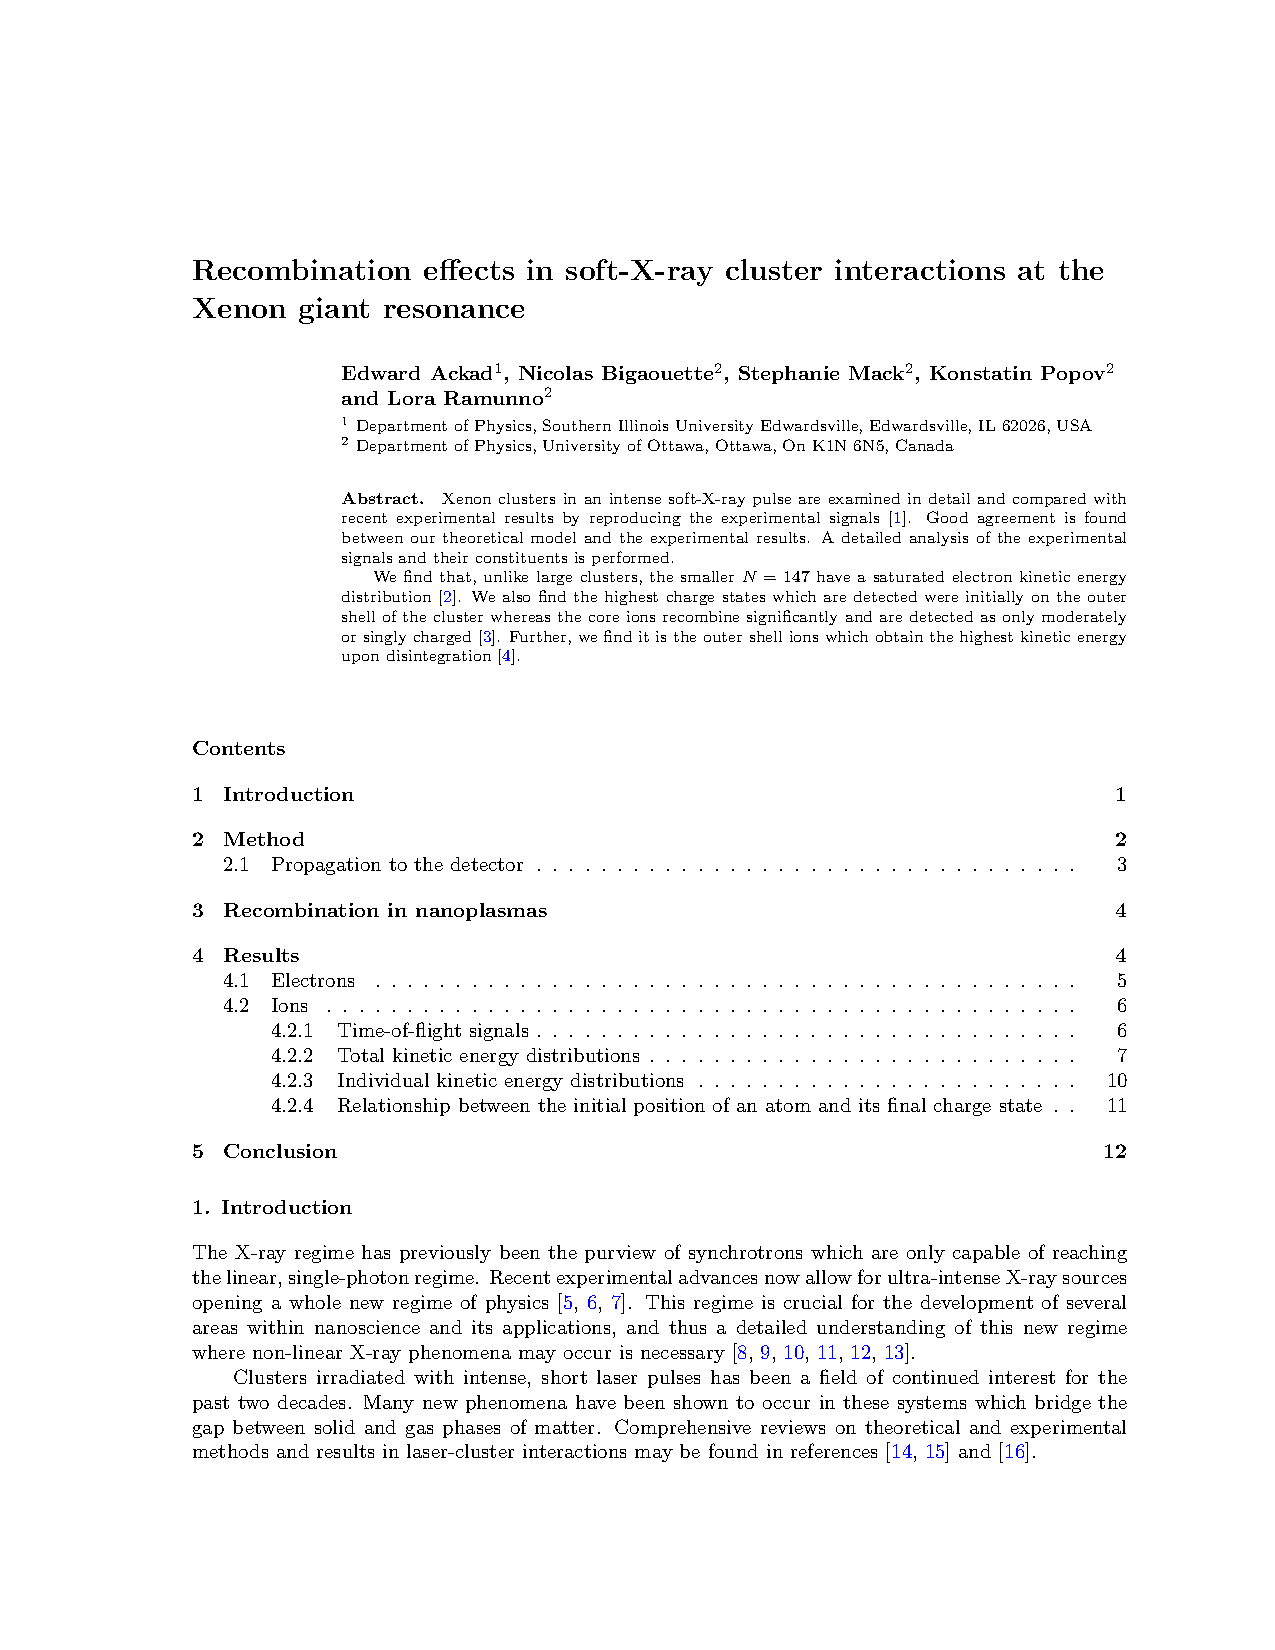
\includepdf[pages=2-,
            addtotoc={
                % Original PDF page, TOC Section hierarchy, # matching TOC level, TOC label, \label{}
                % http://cs.brown.edu/system/software/latex/doc/pdfpages.pdf
                2,subsection,2,Abstract,paper_recomb_abstract,
                3,subsection,2,Contents,paper_recomb_contents,
                3,subsection,2,Introduction,paper_recomb_intro,
                4,subsection,2,Method,paper_recomb_method,
                5,subsubsection,3,Propagation to the detector,paper_recomb_method_propagation,
                6,subsection,2,Recombination in nanoplasmas,paper_recomb_recomb,
                7,subsection,2,Results,paper_recomb_results,
                7,subsubsection,3,Electrons,paper_recomb_results_elec,
                8,subsubsection,3,Ions,paper_recomb_results_ions,
                9,paragraph,4,Time-of-flight signals,paper_recomb_results_ions_tof,
                11,paragraph,4,Total kinetic energy distributions,paper_recomb_results_ions_k_tot,
                13,paragraph,4,Individual kinetic energy distributions,paper_recomb_results_ions_k_ind,
                15,paragraph,4,Relationship between the initial position of an atom and its final charge state,paper_recomb_results_ions_cs,
                16,subsection,2,Conclusion,paper_recomb_conclusion,
                16,subsection,2,Acknowledgments,paper_recomb_ack,
                16,subsection,2,References,paper_recomb_refs
            }]{papers/Ackad2013_Recomb.pdf}
